\section{Проектирование}

\subsection{Таблицы с описанием таблиц базы данных}

В таблицах~\ref{tab:employee_type}--\ref{tab:geo_request} представлены атрибуты таблиц базы данных геомониторинга.
Каждая таблица с описанием содержит колонки: номер по порядку, имя атрибута на русском и английском языках, тип атрибута, при необходимости со значением размера, значение по умолчанию, признак ключа при наличии, для внешнего ключа ссылка на таблицу, примечание.

% Настройка стилей колонок для выравнивания как на картинке
\newcolumntype{Y}{>{\centering\arraybackslash}X} % Растягиваемая колонка по центру
\newcolumntype{Z}{>{\raggedright\arraybackslash}X} % Растягиваемая по левому краю (для длинных названий)
\newcolumntype{C}[1]{>{\centering\arraybackslash}p{#1}} % Фиксированная ширина по центру


% --- Таблица 1: employee_type ---
\begin{table}[H]
    \caption{Типы сотрудников}
    \label{tab:employee_type}
    \footnotesize % Уменьшенный шрифт для вместимости
    \renewcommand{\arraystretch}{1.3} % Чуть больше отступ между строками
    \begin{tabularx}{\textwidth}{|c Z Y C{2.2cm} c c c c|}
        \hline
        \multicolumn{8}{|c|}{\textbf{Тип сотрудника -- employee\_type}} \\
        \hline
        № & Название RU & Название EN & Тип атрибута & Def & Тип ключа & Ссылка & Прим. \\
        \hline
        1 & тип\_сотрудника\_id & employee\_type\_id & INT & - & PK & - & NOT NULL \\
        2 & название\_типа & name & VARCHAR(50) & - & UQ & - & NOT NULL \\
        3 & описание & description & TEXT & NULL & - & - & NULL \\
        \hline
    \end{tabularx}
\end{table}

% --- Таблица 2: employee ---
\begin{table}[H]
    \caption{Таблица сотрудников}
    \label{tab:employee}
    \footnotesize
    \renewcommand{\arraystretch}{1.3}
    \begin{tabularx}{\textwidth}{|c Z Y C{2.2cm} c c c c|}
        \hline
        \multicolumn{8}{|c|}{\textbf{Сотрудник -- employee}} \\
        \hline
        № & Название RU & Название EN & Тип атрибута & Def & Тип ключа & Ссылка & Прим. \\
        \hline
        1 & сотрудник\_id & employee\_id & INT & - & PK & - & NOT NULL \\
        2 & тип\_сотрудника\_id & employee\_type\_id & INT & - & FK & empl\_type & NOT NULL \\
        3 & фио & full\_name & VARCHAR(255) & - & - & - & NOT NULL \\
        4 & логин & login & VARCHAR(50) & - & UQ & - & NOT NULL \\
        5 & статус & status & VARCHAR(30) & - & - & - & NOT NULL \\
        6 & должность & position & VARCHAR(50) & - & - & - & NOT NULL \\
        \hline
    \end{tabularx}
\end{table}

% --- Таблица 3: parking_zone ---
\begin{table}[H]
    \caption{Таблица зон парковки}
    \label{tab:parking_zone}
    \footnotesize
    \renewcommand{\arraystretch}{1.3}
    \begin{tabularx}{\textwidth}{|c Z Y C{2.2cm} c c c c|}
        \hline
        \multicolumn{8}{|c|}{\textbf{Зона парковки -- parking\_zone}} \\
        \hline
        № & Название RU & Название EN & Тип атрибута & Def & Тип ключа & Ссылка & Прим. \\
        \hline
        1 & зона\_парковки\_id & parking\_zone\_id & INT & - & PK & - & NOT NULL \\
        2 & название & name & VARCHAR(100) & - & - & - & NOT NULL \\
        3 & тип\_зоны & zone\_type & VARCHAR(30) & - & - & - & NOT NULL \\
        4 & район\_города & city\_district & VARCHAR(100) & - & - & - & NOT NULL \\
        5 & макс\_авто & max\_cars & INT & - & - & - & NOT NULL \\
        6 & статус & active\_status & VARCHAR(30) & - & - & - & NOT NULL \\
        \hline
    \end{tabularx}
\end{table}

% --- Таблица 4: parking_zone_point ---
\begin{table}[H]
    \caption{Координаты зон парковки}
    \label{tab:parking_zone_point}
    \footnotesize
    \renewcommand{\arraystretch}{1.3}
    \begin{tabularx}{\textwidth}{|c Z Y C{2.2cm} c c c c|}
        \hline
        \multicolumn{8}{|c|}{\textbf{Координаты зоны парковки -- parking\_zone\_point}} \\
        \hline
        № & Название RU & Название EN & Тип атрибута & Def & Тип ключа & Ссылка & Прим. \\
        \hline
        1 & координаты\_зоны\_id & parking\_zone\_point\_id & INT & - & PK & - & NOT NULL \\
        2 & зона\_парковки\_id & parking\_zone\_id & INT & - & FK & park\_zone & NOT NULL \\
        3 & номер\_вершины & vertex\_number & INT & - & - & - & NOT NULL \\
        4 & широта & latitude & NUMERIC(9,6) & - & - & - & NOT NULL \\
        5 & долгота & longitude & NUMERIC(9,6) & - & - & - & NOT NULL \\
        \hline
    \end{tabularx}
\end{table}

% --- Таблица 5: car ---
\begin{table}[H]
    \caption{Таблица автомобилей}
    \label{tab:car}
    \footnotesize
    \renewcommand{\arraystretch}{1.3}
    \begin{tabularx}{\textwidth}{|c Z Y C{2.2cm} c c c c|}
        \hline
        \multicolumn{8}{|c|}{\textbf{Автомобиль -- car}} \\
        \hline
        № & Название RU & Название EN & Тип атрибута & Def & Тип ключа & Ссылка & Прим. \\
        \hline
        1 & авто\_id & car\_id & INT & - & PK & - & NOT NULL \\
        2 & зона\_парковки\_id & parking\_zone\_id & INT & NULL & FK & park\_zone & NULL \\
        3 & гос\_номер & reg\_number & VARCHAR(20) & - & UQ & - & NOT NULL \\
        4 & марка & brand & VARCHAR(100) & - & - & - & NOT NULL \\
        5 & модель & model & VARCHAR(100) & - & - & - & NOT NULL \\
        6 & год\_выпуска & manufacture\_year & INT & - & - & - & NOT NULL \\
        7 & vin\_номер & vin & VARCHAR(17) & - & UQ & - & NOT NULL \\
        8 & статус & current\_status & VARCHAR(30) & - & - & - & NOT NULL \\
        \hline
    \end{tabularx}
\end{table}

% --- Таблица 6: movement_track ---
\begin{table}[H]
    \caption{Таблица треков движения}
    \label{tab:movement_track}
    \footnotesize
    \renewcommand{\arraystretch}{1.3}
    \begin{tabularx}{\textwidth}{|c Z Y C{2.2cm} c c c c|}
        \hline
        \multicolumn{8}{|c|}{\textbf{Трек движения -- track}} \\
        \hline
        № & Название RU & Название EN & Тип атрибута & Def & Тип ключа & Ссылка & Прим. \\
        \hline
        1 & трек\_id & track\_id & INT & - & PK & - & NOT NULL \\
        2 & авто\_id & car\_id & INT & - & FK & car & NOT NULL \\
        3 & время\_начала & start\_time & TIMESTAMP & - & - & - & NOT NULL \\
        4 & время\_конца & end\_time & TIMESTAMP & NULL & - & - & NULL \\
        5 & статус\_трека & track\_status & VARCHAR(30) & - & - & - & NOT NULL \\
        6 & вид\_трека & track\_kind & VARCHAR(30) & - & - & - & NOT NULL \\
        \hline
    \end{tabularx}
\end{table}

% --- Таблица 7: track_point ---
\begin{table}[H]
    \caption{Точки трека движения}
    \label{tab:track_point}
    \footnotesize
    \renewcommand{\arraystretch}{1.3}
    \begin{tabularx}{\textwidth}{|c Z Y C{2.2cm} c c c c|}
        \hline
        \multicolumn{8}{|c|}{\textbf{Координаты точки трека -- track\_point}} \\
        \hline
        № & Название RU & Название EN & Тип атрибута & Def & Тип ключа & Ссылка & Прим. \\
        \hline
        1 & координаты\_точки\_id & track\_point\_id & INT & - & PK & - & NOT NULL \\
        2 & трек\_id & track\_id & INT & - & FK & mov\_track & NOT NULL \\
		3 & авто\_id & car\_id & INT & - & FK & car & NULL \\
        4 & широта & latitude & NUMERIC(9,6) & - & - & - & NOT NULL \\
        5 & долгота & longitude & NUMERIC(9,6) & - & - & - & NOT NULL \\
        6 & скорость & speed\_kmh & NUMERIC(6,2) & NULL & - & - & NULL \\
        7 & источник\_данных & data\_source & VARCHAR(30) & - & - & - & NOT NULL \\
        \hline
    \end{tabularx}
\end{table}

% --- Таблица 8: alert_event ---
\begin{table}[H]
    \caption{Таблица тревожных событий}
    \label{tab:alert_event}
    \footnotesize
    \renewcommand{\arraystretch}{1.3}
    \begin{tabularx}{\textwidth}{|c Z Y C{2.2cm} c c c c|}
        \hline
        \multicolumn{8}{|c|}{\textbf{Тревожное событие -- alert\_event}} \\
        \hline
        № & Название RU & Название EN & Тип атрибута & Def & Тип ключа & Ссылка & Прим. \\
        \hline
        1 & событие\_id & alert\_event\_id & INT & - & PK & - & NOT NULL \\
        2 & авто\_id & car\_id & INT & - & FK & car & NOT NULL \\
        3 & сотрудник\_id & employee\_id & INT & NULL & FK & employee & NULL \\
        4 & тип\_события & event\_type & VARCHAR(50) & - & - & - & NOT NULL \\
        5 & широта & latitude & NUMERIC(9,6) & NULL & - & - & NULL \\
        6 & долгота & longitude & NUMERIC(9,6) & NULL & - & - & NULL \\
        7 & описание & description & TEXT & NULL & - & - & NULL \\
        8 & статус\_обработки & process\_status & VARCHAR(30) & - & - & - & NOT NULL \\
        \hline
    \end{tabularx}
\end{table}

% --- Таблица 9: geo_request ---
\begin{table}[H]
    \caption{Таблица обращений}
    \label{tab:geo_request}
    \footnotesize
    \renewcommand{\arraystretch}{1.3}
    \begin{tabularx}{\textwidth}{|c Z Y C{2.2cm} c c c c|}
        \hline
        \multicolumn{8}{|c|}{\textbf{Обращение к геомониторингу -- geo\_request}} \\
        \hline
        № & Название RU & Название EN & Тип атрибута & Def & Тип ключа & Ссылка & Прим. \\
        \hline
        1 & запрос\_id & geo\_request\_id & INT & - & PK & - & NOT NULL \\
        2 & сотрудник\_id & employee\_id & INT & - & FK & employee & NOT NULL \\
        3 & авто\_id & car\_id & INT & - & FK & car & NOT NULL \\
        4 & тип\_запроса & request\_type & VARCHAR(50) & - & - & - & NOT NULL \\
        5 & цель\_запроса & request\_goal & TEXT & - & - & - & NOT NULL \\
        \hline
    \end{tabularx}
\end{table}

\subsection{Лингвистическое описание схемы базы данных}

\begin{enumerate}
    \item Тип сотрудника (тип\_сотрудника\_id(INT), название\_типа(VARCHAR(50)), описание(TEXT)).
    
    \item Сотрудник (сотрудник\_id(INT), тип\_сотрудника\_id(INT), фио(VARCHAR(255)), логин(VARCHAR(50)), статус(VARCHAR(30)), должность(VARCHAR(50))).
    
    \item Зона парковки (зона\_парковки\_id(INT), название(VARCHAR(100)),\\ тип\_зоны(VARCHAR(30)), район\_города(VARCHAR(100)), макс\_авто(INT), статус(VARCHAR(30))).
    
    \item Координаты зоны парковки (координаты\_зоны\_id(INT), зона\_парковки\_id(INT), номер\_вершины(INT), широта(NUMERIC(9,6)), долгота(NUMERIC(9,6))).
    
    \item Автомобиль (авто\_id(INT), зона\_парковки\_id(INT), гос\_номер(VARCHAR(20)), марка(VARCHAR(100)), модель(VARCHAR(100)), год\_выпуска(INT), \\ vin\_номер(VARCHAR(17)), статус(VARCHAR(30))).
    
    \item Трек движения (трек\_id(INT), авто\_id(INT), время\_начала(TIMESTAMP), время\_конца(TIMESTAMP), статус\_трека(VARCHAR(30)), \\вид\_трека(VARCHAR(30))).
    
    \item Координаты точки трека (координаты\_точки\_id(INT), трек\_id(INT), широта(NUMERIC(9,6)), долгота(NUMERIC(9,6)), скорость(NUMERIC(6,2)), источник\_данных(VARCHAR(30))).
    
    \item Тревожное событие (событие\_id(INT), авто\_id(INT), сотрудник\_id(INT), \\ тип\_события(VARCHAR(50)), широта(NUMERIC(9,6)), долгота(NUMERIC(9,6)), описание(TEXT), статус\_обработки(VARCHAR(30))).
    
    \item Обращения к геомониторингу (запрос\_id(INT), сотрудник\_id(INT), авто\_id(INT), тип\_запроса(VARCHAR(50)), цель\_запроса(TEXT)).
\end{enumerate}

\begin{figure}[h!]
\centering
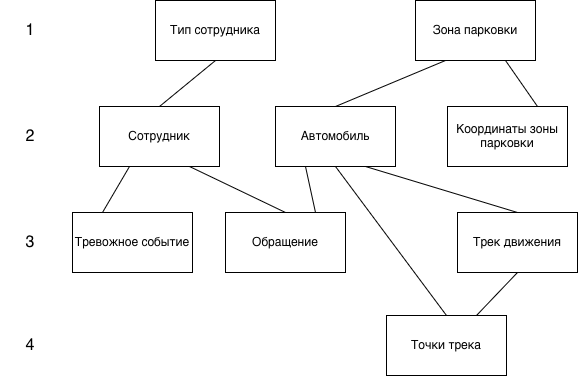
\includegraphics[width=0.9\textwidth]{myPhoto/levels.png}
\caption{Уровни заполнения базы данных}
\end{figure}
\newpage

\clearpage
\newgeometry{paperwidth=420mm,paperheight=297mm,margin=-2mm}
\begin{landscape}
  \thispagestyle{empty}
  \captionsetup{font=small,skip=4pt}

  \begin{figure}[!p]
    \centering
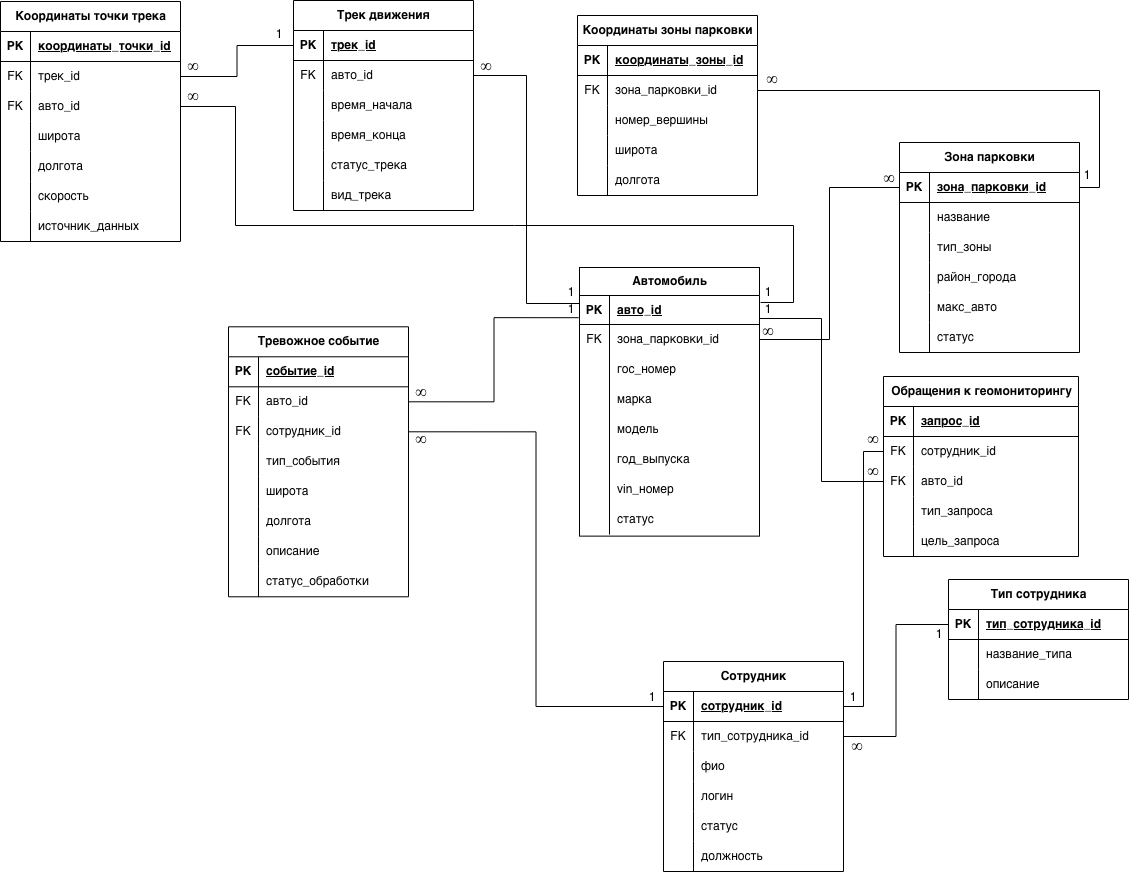
\includegraphics[width=\linewidth,height=\dimexpr\textheight-4\baselineskip\relax,keepaspectratio]{myPhoto/db-russia.png}
    \caption{Графическое описание схемы базы данных на русском языке}
    \label{fig:placeholder}
  \end{figure}
\end{landscape}

\restoregeometry
\clearpage

\clearpage
\newgeometry{paperwidth=420mm,paperheight=297mm,margin=-2mm}
\begin{landscape}
  \thispagestyle{empty}
  \captionsetup{font=small,skip=4pt}

  \begin{figure}[!p]
    \centering
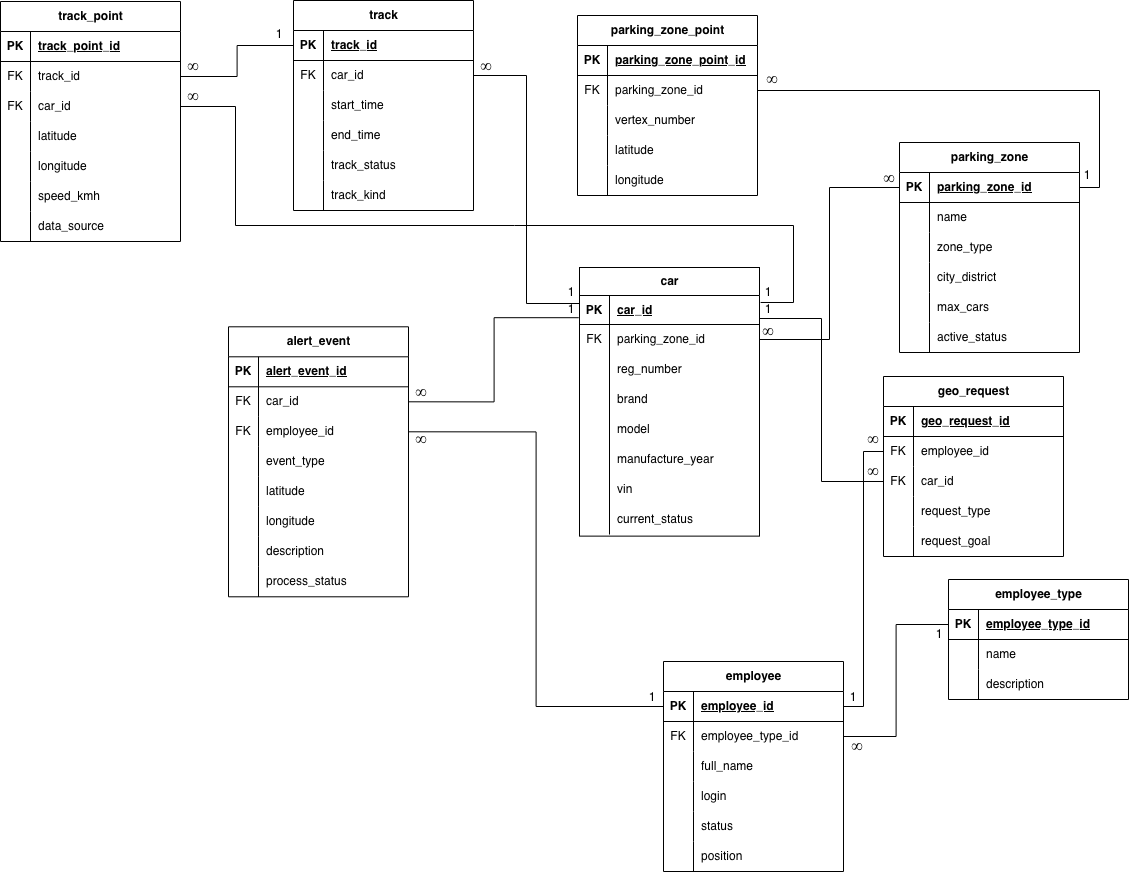
\includegraphics[width=\linewidth,height=\dimexpr\textheight-4\baselineskip\relax,keepaspectratio]{myPhoto/db-english.png}
    \caption{Графическое описание схемы базы данных на английском языке}
    \label{fig:placeholder}
  \end{figure}
\end{landscape}

\restoregeometry
\clearpage

\subsection{Исходный текст программы генерации схемы базы данных}

База данных создана средствами СУБД PostgreSQL с использованием SQL-скриптов, приведенных в \hyperref[app:A]{приложении A} (схема на рис. 3).

Наполнение базы синтетическими данными (320225 записей в 9 таблицах) выполнено утилитой на языке Go 1.25.4 с использованием драйвера pgx. Таблицы-справочники заполнены статическими данными, а основные сущности сгенерированы алгоритмически с учетом логических связей в \hyperref[app:B]{приложении Б}.

\newpage